% Everyone should proof read this
% Anurag PR Complete 1
% Akshay PR Complete 1

\chapter{Conclusion} \label{Chapter:sixth} 
With little to no knowledge and direct hands-on experience in the development of Industry 4.0 technology or Cloud-Based Computing prior to the assignment of this project, we aimed to establish an End-to-End wireless telemetry system to automate the improvement of wireless communication. More specifically in terms of data transportation and data throughput, aligning with the growing industry demand of 5G, intelligent data collection, processing, ML Inferences, and Predictive capabilities at the Edge- and at the Cloud-Level. Industry 4.0 aims to inter-connect and computerize the traditional manufacturing and production system in the industrial services, improving the automation and operational efficiency. This communication between machines resulting to the Internet and IoT connectivity, which are the technology basis in Industry 4.0. 5G communication standard automatically become the requirement in the application of industry 4.0, providing low latency connectivity between devices or machines resulting in high-speed data transmission, while ensuring the safety and controls over the network. Contributing to the studies of Industry 4.0, our project focuses on developing a wireless system with edge technology, reducing the data transmission time, improving the performance through the  Over-the-Top (OTT) application, which is to be accomplished as a future work. 

With the assistance and applications provided by InterDigital and Amazon Web Service (AWS), the initial plans and research of the project managed to reach most of the milestone set out in the project brief. Wide variety of features on AWS, give upper hands in using the services provided such as S3 bucket, functioning as the fundamental data storage, IoT Greengrass which deploy edge native application to the edge nodes, SageMaker to build and train the ML model, deploying the intelligence in the proximity of IoT devices at the edge of network, reducing the latency and data transmission across the network. Alongside these services, AdvantEDGE, a mobile edge emulation platform, which have yet to be implemented fully in the project, offers so much more in the technology of edge computing. It provides an environment to simulate and test the network model which can be connected to the real edge application, foreseeing the potential and improvement to be made for the designed wireless system. Demonstrating the project in the form of an OTT application would require more resources to complete, however as the entire document concludes, edge computing really proves to be the stepping stone for the 5G wireless communication and for the future application of standard Industry 4.0 practices.



\section{Achievement} 
The specification that was written at the start of the project can be found in Appendix \ref{appendix:project_specification}. The specification demands several deliverables from the project and the evaluation of these deliverables will now be discussed.

\subsection{Deliverable I - Router Data/Transmission Specific:}
\begin{figure}[ht]
    \centering
    \fbox{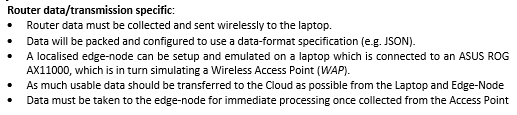
\includegraphics[width=1\linewidth]{pages/Chapter6/Chapter 6 Images/router_data_spec.png}}
    \caption{Deliverables for Router Data/Transmission Specification points taken from the Project Specification}
    \label{fig:router_data_deliverables}
\end{figure}

The first set of deliverables addresses data collection and transmission. The data needs to be retrieved through wireless methods through the Wireless Access Point, which in this project is the  ASUS ROG GT-AX11000 Router. The data must then converted to JSON format as this was proven to be the best format for transportation as discussed in Section \ref{Section: Database File Conversion}. This was accomplished successfully and data transformation is handled for the best format at every front. Either in the direct pipeline to the cloud from the laptop, or at the Edge Node where processing capabilities frees the End-User device. The edge node was also successfully deployed to a virtual machine simulating separate hardware running at the edge Location, via the usage of AWS IoT Greengrass and AWS IoT Core. Developments were also made into InterDigital's AdvantEdge as a method of deploying edge nodes, however there were issues with the containerisation of ETL functions to deploy into AdvantEdge's network models and hence the full edge node via AdvantEdge could not be explored, but via Greengrass the full edge-node was deployed. As per the last deliverable in this list, the data is also taken immediately via a shared network folder between the user-endpoint and the edge-node, allowing for immediate transfer.

\subsection{Deliverable II - AWS Data Lake and ML Tools}
\begin{figure}[ht]
    \centering
    \fbox{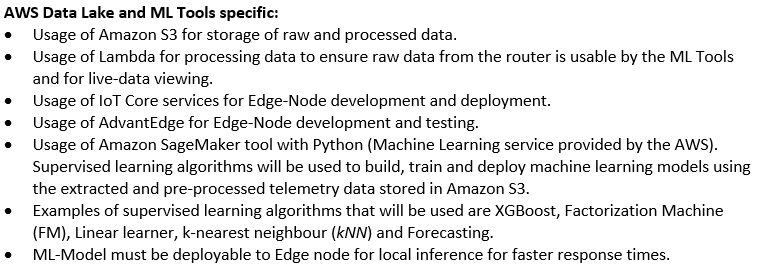
\includegraphics[width=1\linewidth]{pages/Chapter6/Chapter 6 Images/edge_aws_spec.png}}
    \caption{Deliverables for Edge Technologies and AWS Data Lake}
    \label{fig:aws_edge_spec}
\end{figure}

The second set of deliverables addresses AWS and edge node technologies as seen in Figure \ref{fig:aws_edge_spec}. As per the first point, the project does correctly use AWS S3 buckets for raw and processed data storage. It is also used for storage of ML Models deployed after training and validation. Lambda functions are correctly used for cloud-based processing, compressing the JSON data tables into a single file for easier processing. Lambda functions are also deployed to each Greengrass edge node. The project explores edge node deployment via both AWS Greengrass with IoT Core as well as through the usage of InterDigital's AdvantEdge edge node solution. There was great success using Greengrass and deployment of cloud-based functions for localised and remote areas with limited access to the cloud, however while the setup and installation of AdvantEdge was completed successfully, the project did not get to a point to develop a container with all the ETL scripts within which stopped edge node deployment with AdvantEdge. 

Then AWS Sagemaker was used successfully as per the specification and correctly helped to analyse useful data, as well as train and develop a model for verification and then deployment of the model. The model was successfully developed using XGBoost as well as kNN algorithms. The XGBoost model proved the best as shown in the ML Section \ref{xgboost-training} and so was deployed to the Greengrass Edge Node successfully. Function duration and comparisons were made to show that a localised model was completed as well proving that the Local-ML was much faster than sending the data to the Cloud for inference purposes. This is proved in the later Results Section.

\subsection{Deliverable III - Over-the-Top Application Specific}
\begin{figure}[ht]
    \centering
    \fbox{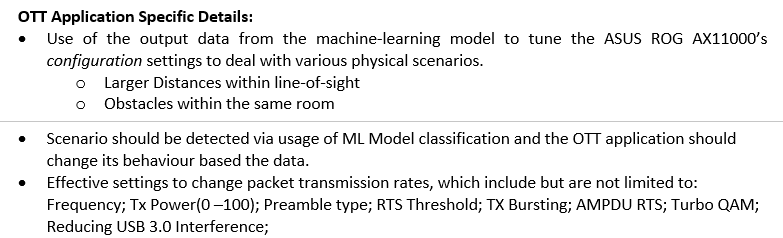
\includegraphics[width=1\linewidth]{pages/Chapter6/Chapter 6 Images/ott_spec.png}}
    \caption{Caption}
    \label{fig:ott_spec}
\end{figure}

The last section of the deliverables covers the final aspect of the project regarding the OTT Application. No deliverable was specifically produced to use the outputs from the ML Model's classification. However, from the start of the project it was known that the OTT Application would always be a last step, and would be dependent on any insights gained from the collected data and based on the ML-Model. Different scenarios were emulated in terms of data throughput, however these were done via software rather than different environment setups as this would provide us with better data to work with and verify model classifications. This emulation of different scenarios with different data throughput rates is discussed in Section \ref{Section: Testing Data Retrieval}. Research was also conducted into the possible router configurations, however no developed was made into changing router configurations via the various ways to access the router configurations. This has been added under future work for this project. The data does not specifically allow for an OTT application to be considered for only one router use-case, as the ML model uses channel stats which is access-point specific data. Any OTT application that we would have considered would have been based on using multiple routers or Access points and implementing some optimisations to each router based on its data throughput. 

\subsection {Deliverable IV - Stretch Goals}
\begin{figure}[ht]
    \centering
    \fbox{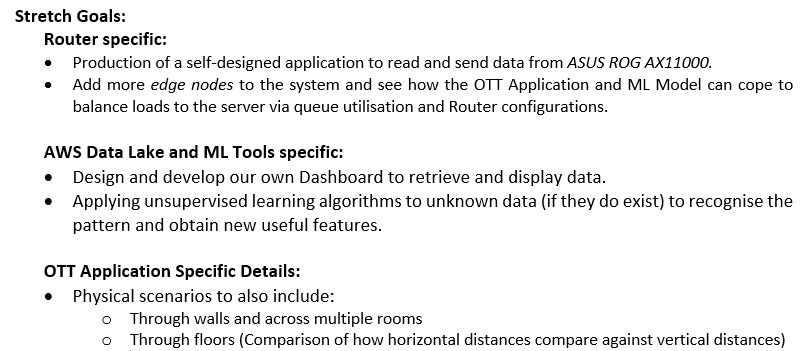
\includegraphics[width=1\linewidth]{pages/Chapter6/Chapter 6 Images/stretch_goals_spec.png}}
    \caption{List of Stretch Goals taken from Specification Document}
    \label{fig:stretch_goals_spec}
\end{figure}
The stretch goals were split into the same sections as per the system design and above project deliverables. Each section would have a goal to focus on upon work completion. Since some stages were finished before the end of the project, resources were available to develop the stretch goals. 

\subsubsection{Router Specific}
\begin{itemize}
    \item A self-designed application was designed and developed to retrieve router data using SSH as well as two separate web-scraper applications rather than the pre-existing Web GUI from ASUS or any other 3rd party application.
    \item Edge Nodes were deployed to two different locations with the ability to deploy separate models to both locations. However, the nodes were completely isolated from each other so no interaction in terms of load-balancing or other were applied.
\end{itemize}

\subsubsection{AWS Data Lake and ML Tools Specific}
\begin{itemize}
    \item Own dashboard to view data was designed and developed. This was done in the form of a web-server and became more useful for validation of results than using Cloud-based analytics as it was quicker for edge-based functions.
    \item No unsupervised algorithms were used, and instead two supervised algorithms were tested for rigorousness.
\end{itemize}

\subsubsection{OTT Application Specific Details}
No further scenarios were tested outside of the conditions for \textit{data throughput} were tested.

As a final conclusion for the achievements of this project. A large majority of the initial deliverables assigned and even stretch goals have been achieved and attribute to the success of the project. While a major impact was had by delayed access to AWS until Weeks 10-11 of the project (as is discussed further in the Project Setbacks section), the project members were still able to develop the project further despite the conditions. 

\section{Project Setbacks} \label{section:Project Setbacks}
While there was great success within the project in all stages, there were also setbacks that were outside of the group's control that impacted the project and they will be discussed within this section.

\paragraph{Impact due to Covid}
At the time of this Group Design Project, the University and many of the aspects of the students' lives were impacted by effects of the COVID-19 Pandemic. Firstly, as this was primarily a software project, a lot of the work required the project members to work on their own laptops and PCs available to them. Progress slowed as hardware constraints were hit especially with the Edge Deployment for both Greengrass and AdvantEdge. Communication had to be completely moved to an online work-space with no direct face-to-face which was a brand new experience for the team as a whole and required getting used to and would impact the psyche of team members. Working from home also meant that the project members would have to often balance a work-life balance and maintaining this can often be challenging especially considering student mental health during the Pandemic. No severe impact to any project members' life was seen within the project but attributes to the successful capabilities of the project members to persevere during this time despite any and all surrounding circumstances without an official workplace.

\paragraph{AWS Setbacks}
For the project, the availability and sponsorship of AWS Access was to be provided. However, there were delays outside of either InterDigital's control or the group's, which meant there were big delays with access to services for member training, development of the project and eventual deployment. Initially, the project members setup and used their own AWS accounts, however after the free trial ran out for many of the services, including S3, Sagemaker and EC2, the members began to be charged and so project development had to be halted immediately. There were discussions in using the project budget, however these funds would have to be approved at several stages. Fortunately, by this time InterDigital were able to provide the AWS access and project development continued around Week 10-11, but still proved to be a big hurdle for the project members to handle. 






% Introduction:
% Need to just make sure technical objectives match up with specification document

% Just check wording here

% Still need to edit just a bit 2.3 edge tech background research


% 3.1 router data complete
% 3.2 good
% 3.3 good
% 3.4 good

% 4_1 router data
% 4_3_Like previously we have implementation api gateway gateway end point but this time for sagemaker rather than s3,

% Change mqqt to mqtt

% 5_1 router data testing is fine,
% Check 5_2 remote-ml lambda fn

% future work:
% Ott applicaiton - ssh to change network settings
% ssh from the edge node directly
% sending timing data from laptop to cloud to edge
% advantedge python script deployment
% the scability solution, with model retraining, and redeployment to different environments with all different models.

% ML - use data from other bands

% Gantt Chart still to be added to project management section

% user manual
% abstract and acknowledgement section still to do
% abstract

% be careful of word limit

% project directory listing

% sort out the appendix orders 

% https://sotonac.sharepoint.com/_layouts/15/sharepoint.aspx
%is teams being weird for you? no documents are loading for me. okay

\section{Results} 
%BTW I haven't shown any real-time application testing, I showed me manually dragging files in in the testing section for the web-app. And said the results section would show the real time ml inference from live data feed. 

%Yeah that would be perfect. Show the tool you use to set the data bandwidth, and then show how the classification matches. That's probably all you need to do to show the result of the edge-node and localised ml model.




As discussed in Section \ref{Section: Testing Data Retrieval}, the data retrieval can be reliably conducted using the SSH method every five seconds which is in line with the minimum sampling interval of the ASUS router data collection feature. With live data testing performed the program was able to smoothly handle the constant incoming stream of new database files all increasing in file size because the latest timestamp datasets are appended to the existing file. Appendix \ref{appendix:Results} shows the screen-captures of the web application and the StarTrinity CST software used to vary the data throughput values. As shown, the web application displays the data throughput value per timestamp in the live graph and the table below shows the live data parameter values along with the machine learning classification. Every classification was tested and the machine learning model was able to correctly classify the data every time. The figure in Section \ref{appendix:Boundarydata} of Appendix \ref{appendix:Results}, also shows that the machine learning model is able to accurately classify the data on the boundary of two classifications (moderate \& strong). 
%More thorough results section required for web app

From the results obtained in Section \ref{Section: Testing Phase of ML Model}, a successful machine learning model for both the k-Nearest Neighbour and XGBoost supervised learning algorithms was built. The model is able to classify data throughput strength of five different classes which are very weak, weak, moderate, strong and very strong. The accuracy achieved by the classifier with the k-Nearest Neighbour algorithm is 98.6\%. This accuracy obtained improved from an accuracy of 89.2\% after more data was collected to retrain the data throughput strength classifier. 

For the XGBoost model built with the Sagemaker Python SDK, it achieved roughly the same accuracy with the k-NN algorithm which is about 98.4\%. The accuracy of this classifier improved drastically from an accuracy of less than 30\% after the retraining of the model using a larger dataset. After achieving a satisfying performance, the XGBoost classifier with the 98.4\% was deployed and the endpoint was used to predict new test data. By making use the API Gateway and AWS Lambda services, the model endpoint was able to predict new test data via the Postman HTTP web service successfully. 
% Here we can discuss the actual results, being the timings of the lambda functions and how quickly they function, the timing of the laptop to the cloud services, the success rate of the ML, the application of advantedge and how that was not succesful etc...

\section{Feedback}

% Include here the feedback from interdigital and their happiness reviews